\documentclass{minimal}
\usepackage{graphicx,color}
\usepackage[utf8]{inputenc}
\usepackage[papersize={648.00bp,288.00bp},text={648.00bp,288.00bp}]{geometry}
\begin{document}
\centering
% Title: gl2ps_renderer figure
% Creator: GL2PS 1.4.2, (C) 1999-2020 C. Geuzaine
% For: Octave
% CreationDate: Tue Feb  8 21:02:35 2022
\setlength{\unitlength}{1pt}
\begin{picture}(0,0)
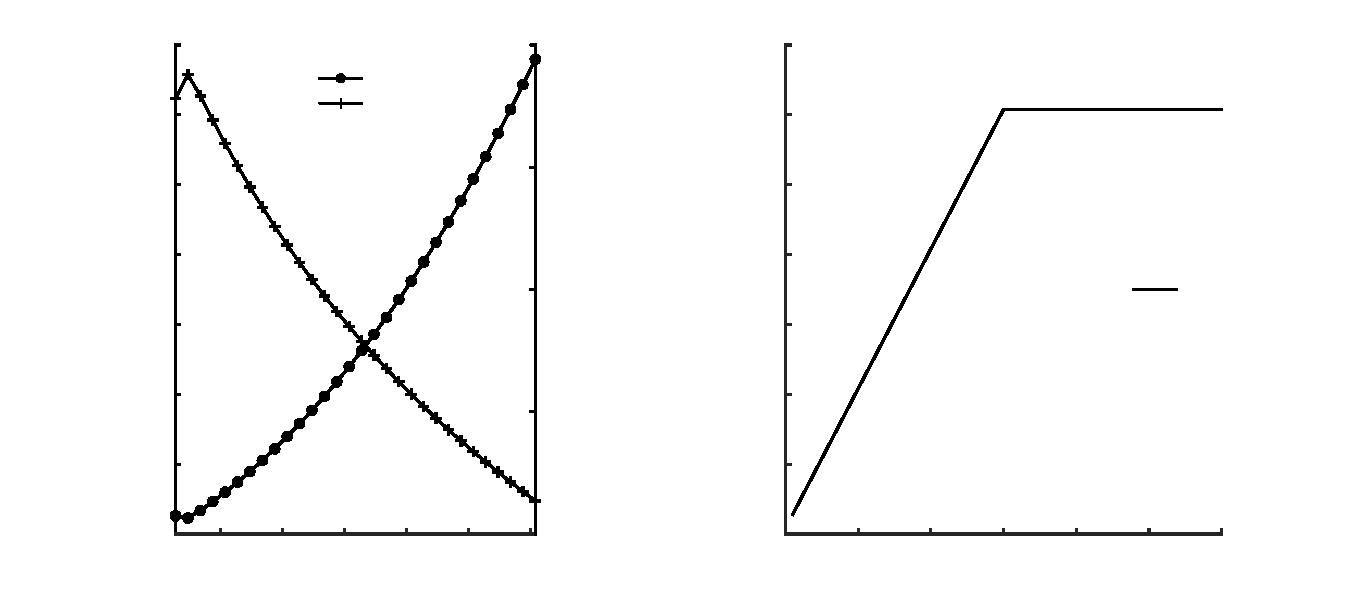
\includegraphics[scale=1]{diamtroDe2-inc}
\end{picture}%
\begin{picture}(648,288)(0,0)
\fontsize{10}{0}\selectfont\put(105.68,24.1889){\makebox(0,0)[t]{\textcolor[rgb]{0.15,0.15,0.15}{{30}}}}
\fontsize{10}{0}\selectfont\put(135.457,24.1889){\makebox(0,0)[t]{\textcolor[rgb]{0.15,0.15,0.15}{{35}}}}
\fontsize{10}{0}\selectfont\put(165.234,24.1889){\makebox(0,0)[t]{\textcolor[rgb]{0.15,0.15,0.15}{{40}}}}
\fontsize{10}{0}\selectfont\put(195.012,24.1889){\makebox(0,0)[t]{\textcolor[rgb]{0.15,0.15,0.15}{{45}}}}
\fontsize{10}{0}\selectfont\put(224.789,24.1889){\makebox(0,0)[t]{\textcolor[rgb]{0.15,0.15,0.15}{{50}}}}
\fontsize{10}{0}\selectfont\put(254.566,24.1889){\makebox(0,0)[t]{\textcolor[rgb]{0.15,0.15,0.15}{{55}}}}
\fontsize{10}{0}\selectfont\put(79.2484,31.68){\makebox(0,0)[r]{\textcolor[rgb]{0,0,0}{{2}}}}
\fontsize{10}{0}\selectfont\put(79.2484,65.2114){\makebox(0,0)[r]{\textcolor[rgb]{0,0,0}{{4}}}}
\fontsize{10}{0}\selectfont\put(79.2484,98.7429){\makebox(0,0)[r]{\textcolor[rgb]{0,0,0}{{6}}}}
\fontsize{10}{0}\selectfont\put(79.2484,132.274){\makebox(0,0)[r]{\textcolor[rgb]{0,0,0}{{8}}}}
\fontsize{10}{0}\selectfont\put(79.2484,165.806){\makebox(0,0)[r]{\textcolor[rgb]{0,0,0}{{10}}}}
\fontsize{10}{0}\selectfont\put(79.2484,199.337){\makebox(0,0)[r]{\textcolor[rgb]{0,0,0}{{12}}}}
\fontsize{10}{0}\selectfont\put(79.2484,232.869){\makebox(0,0)[r]{\textcolor[rgb]{0,0,0}{{14}}}}
\fontsize{10}{0}\selectfont\put(79.2484,266.4){\makebox(0,0)[r]{\textcolor[rgb]{0,0,0}{{16}}}}
\fontsize{10}{0}\selectfont\put(170.594,11.1889){\makebox(0,0)[t]{\textcolor[rgb]{0.15,0.15,0.15}{{Diámetro de Tubería D [mm]}}}}
\fontsize{10}{0}\selectfont\put(62.2484,149.04){\rotatebox{90}{\makebox(0,0)[b]{\textcolor[rgb]{0,0,0}{{Caudal Q [L/s]}}}}}
\fontsize{8}{0}\selectfont\put(256.948,259.5){\makebox(0,0)[r]{\textcolor[rgb]{0,0,0}{{$D_e~\displaystyle\longrightarrow$ }}}}
\fontsize{10}{0}\selectfont\put(105.68,24.1889){\makebox(0,0)[t]{\textcolor[rgb]{0.15,0.15,0.15}{{30}}}}
\fontsize{10}{0}\selectfont\put(135.457,24.1889){\makebox(0,0)[t]{\textcolor[rgb]{0.15,0.15,0.15}{{35}}}}
\fontsize{10}{0}\selectfont\put(165.234,24.1889){\makebox(0,0)[t]{\textcolor[rgb]{0.15,0.15,0.15}{{40}}}}
\fontsize{10}{0}\selectfont\put(195.012,24.1889){\makebox(0,0)[t]{\textcolor[rgb]{0.15,0.15,0.15}{{45}}}}
\fontsize{10}{0}\selectfont\put(224.789,24.1889){\makebox(0,0)[t]{\textcolor[rgb]{0.15,0.15,0.15}{{50}}}}
\fontsize{10}{0}\selectfont\put(254.566,24.1889){\makebox(0,0)[t]{\textcolor[rgb]{0.15,0.15,0.15}{{55}}}}
\fontsize{10}{0}\selectfont\put(261.94,31.68){\makebox(0,0)[l]{\textcolor[rgb]{0,0,0}{{0.014}}}}
\fontsize{10}{0}\selectfont\put(261.94,90.36){\makebox(0,0)[l]{\textcolor[rgb]{0,0,0}{{0.015}}}}
\fontsize{10}{0}\selectfont\put(261.94,149.04){\makebox(0,0)[l]{\textcolor[rgb]{0,0,0}{{0.016}}}}
\fontsize{10}{0}\selectfont\put(261.94,207.72){\makebox(0,0)[l]{\textcolor[rgb]{0,0,0}{{0.017}}}}
\fontsize{10}{0}\selectfont\put(261.94,266.4){\makebox(0,0)[l]{\textcolor[rgb]{0,0,0}{{0.018}}}}
\fontsize{10}{0}\selectfont\put(293.94,149.04){\rotatebox{90}{\makebox(0,0)[t]{\textcolor[rgb]{0,0,0}{{Factor de Friccion $f$}}}}}
\fontsize{8}{0}\selectfont\put(256.948,47.576){\makebox(0,0)[r]{\textcolor[rgb]{0,0,0}{{$f_e~\displaystyle\longrightarrow$ }}}}
\fontsize{8}{0}\selectfont\put(177.607,250.387){\makebox(0,0)[l]{\textcolor[rgb]{0,0,0}{{Q}}}}
\fontsize{8}{0}\selectfont\put(177.607,238.383){\makebox(0,0)[l]{\textcolor[rgb]{0,0,0}{{$f$}}}}
\fontsize{10}{0}\selectfont\put(377.007,24.1889){\makebox(0,0)[t]{\textcolor[rgb]{0.15,0.15,0.15}{{0}}}}
\fontsize{10}{0}\selectfont\put(411.913,24.1889){\makebox(0,0)[t]{\textcolor[rgb]{0.15,0.15,0.15}{{10}}}}
\fontsize{10}{0}\selectfont\put(446.818,24.1889){\makebox(0,0)[t]{\textcolor[rgb]{0.15,0.15,0.15}{{20}}}}
\fontsize{10}{0}\selectfont\put(481.724,24.1889){\makebox(0,0)[t]{\textcolor[rgb]{0.15,0.15,0.15}{{30}}}}
\fontsize{10}{0}\selectfont\put(516.629,24.1889){\makebox(0,0)[t]{\textcolor[rgb]{0.15,0.15,0.15}{{40}}}}
\fontsize{10}{0}\selectfont\put(551.535,24.1889){\makebox(0,0)[t]{\textcolor[rgb]{0.15,0.15,0.15}{{50}}}}
\fontsize{10}{0}\selectfont\put(586.44,24.1889){\makebox(0,0)[t]{\textcolor[rgb]{0.15,0.15,0.15}{{60}}}}
\fontsize{10}{0}\selectfont\put(371.997,31.68){\makebox(0,0)[r]{\textcolor[rgb]{0.15,0.15,0.15}{{25}}}}
\fontsize{10}{0}\selectfont\put(371.997,65.2114){\makebox(0,0)[r]{\textcolor[rgb]{0.15,0.15,0.15}{{30}}}}
\fontsize{10}{0}\selectfont\put(371.997,98.7428){\makebox(0,0)[r]{\textcolor[rgb]{0.15,0.15,0.15}{{35}}}}
\fontsize{10}{0}\selectfont\put(371.997,132.274){\makebox(0,0)[r]{\textcolor[rgb]{0.15,0.15,0.15}{{40}}}}
\fontsize{10}{0}\selectfont\put(371.997,165.806){\makebox(0,0)[r]{\textcolor[rgb]{0.15,0.15,0.15}{{45}}}}
\fontsize{10}{0}\selectfont\put(371.997,199.337){\makebox(0,0)[r]{\textcolor[rgb]{0.15,0.15,0.15}{{50}}}}
\fontsize{10}{0}\selectfont\put(371.997,232.869){\makebox(0,0)[r]{\textcolor[rgb]{0.15,0.15,0.15}{{55}}}}
\fontsize{10}{0}\selectfont\put(371.997,266.4){\makebox(0,0)[r]{\textcolor[rgb]{0.15,0.15,0.15}{{60}}}}
\fontsize{10}{0}\selectfont\put(354.997,149.04){\rotatebox{90}{\makebox(0,0)[b]{\textcolor[rgb]{0.15,0.15,0.15}{{Diámetro de Tubería D [mm]}}}}}
\fontsize{10}{0}\selectfont\put(481.724,11.1889){\makebox(0,0)[t]{\textcolor[rgb]{0.15,0.15,0.15}{{Número de iteraciones}}}}
\fontsize{8}{0}\selectfont\put(568.427,149.04){\makebox(0,0)[l]{\textcolor[rgb]{0,0,0}{{D}}}}
\end{picture}
\end{document}
